\documentclass[11pt]{article}
\usepackage[a4paper,margin=2.3cm]{geometry}
\usepackage{amsmath,amssymb,amsthm,mathtools}
\usepackage{graphicx}
\usepackage{booktabs}
\usepackage{array}
\usepackage{microtype}
\usepackage{hyperref}
\usepackage{enumitem}
\usepackage{caption}
\usepackage{float}
\usepackage{xcolor}
\hypersetup{colorlinks=true,linkcolor=black,citecolor=black,urlcolor=blue}
\newtheorem{theorem}{Theorem}
\newtheorem{proposition}{Proposition}
\newtheorem{corollary}{Corollary}
\newtheorem{lemma}{Lemma}
\theoremstyle{remark}\newtheorem{remark}{Remark}
\title{\textbf{From Heavy Spectral Participation to $SU(3)$ Family Holonomy}\\\large Weighted Contractions, Defect Geometry, and Determinant-Locked Transport}
\author{Gregorio Rozas Fernández\\\small Independent Researcher}
\date{Draft for scientific circulation -- September 2026}

\begin{document}
\maketitle

\begin{abstract}
We introduce a contraction-based operator-geometric mechanism by which a non-universal heavy spectrum can generate an exactly determinant-one non-Abelian rank-three connection. Canonical normalization of a positive heavy-participation metric $\Pi$ defines a positive contraction $K=[\Pi(I+\Pi)^{-1}]^{1/2}$. A structural cyclic hop $S$ compresses to the light sector as $B=KSK$. For anisotropic $K$, $B$ is non-normal and the commutator $[B,B^\dagger]$ supplies a distinguished traceless curvature direction. Because $B$ is generically a strict $3\times 3$ contraction, any one-step unitary completion requires at least three complementary dimensions, giving a minimal $3+3$ ambient space. The determinant sector becomes exactly locked when the defect plane is constructed from the anti-Hermitian oriented contraction $C(z)=\epsilon(zB-z^*B^\dagger)$. With $D_C=(I-C^\dagger C)^{1/2}$ and $\Psi_C=(C,D_C)^T$, the canonical Wilczek--Zee connection $A=\Psi_C^\dagger d\Psi_C$ obeys the exact identity
\[
A=\tfrac12\big([dC,C]+[D_C,dD_C]\big),\qquad \mathrm{Tr}\,A=0.
\]
At $z=0$ the curvature is $F(0)=\epsilon^2[B,B^\dagger]dz\wedge dz^*$. The isotropic weighted cycle is exactly flat, whereas generic anisotropy activates all three root sectors at second curvature-jet order. An explicit rational certificate yields eight linearly independent curvature-jet Lie generators; consequently full $\mathfrak{su}(3)$ holonomy occurs on a nonempty open dense subset of the admissible weight space. The resulting chain is
\[
\text{heavy spectrum}\to\text{participation}\to\text{weighted contraction}\to 3+3\text{ defect geometry}\to SU(3)\text{ holonomy}.
\]
We discuss possible relevance to family mixing and determinant-based strong-CP protection, while emphasizing that a physical CKM contour and a complete ultraviolet strong-CP solution are not derived here.
\end{abstract}

\noindent\textbf{Scientific status.} This paper presents a theoretical mathematical construction. It does not report experimental evidence for new particles or interactions. Claims concerning flavor phenomenology are explicitly conditional on an ultraviolet realization and on a derived physical transport path.

\section{Introduction}
Geometric phases convert adiabatic transport into observable phase information. Berry's Abelian construction \cite{Berry1984} and the Wilczek--Zee non-Abelian generalization \cite{WilczekZee1984} established that degenerate subspaces naturally carry matrix-valued geometric connections. The relation between curvature and holonomy is controlled by the Ambrose--Singer theorem \cite{AmbroseSinger1953}. Canonical Stiefel and Grassmann connections have subsequently become standard tools in holonomic quantum control \cite{Tanimura2005}, and three-dimensional non-Abelian holonomy has been realized experimentally \cite{Neef2023}.

Independently, contraction and dilation theory provides a precise language for embedding an apparently dissipative or norm-losing subsystem in a larger unitary system. Julia operators and defect spaces are standard objects in this theory \cite{SzNagy2010,JulaModern2021}. These two mathematical traditions---unitary dilation and non-Abelian geometric transport---are usually developed separately.

The construction proposed here links them through a third ingredient: a positive participation metric generated by a gapped heavy sector. The basic question is whether heavy spectral anisotropy can become non-Abelian family orientation without inserting an arbitrary family rotation by hand.

The answer is affirmative at the level of operator geometry. The central chain is illustrated in Fig.~\ref{fig:pipeline}.

\begin{figure}[H]
\centering
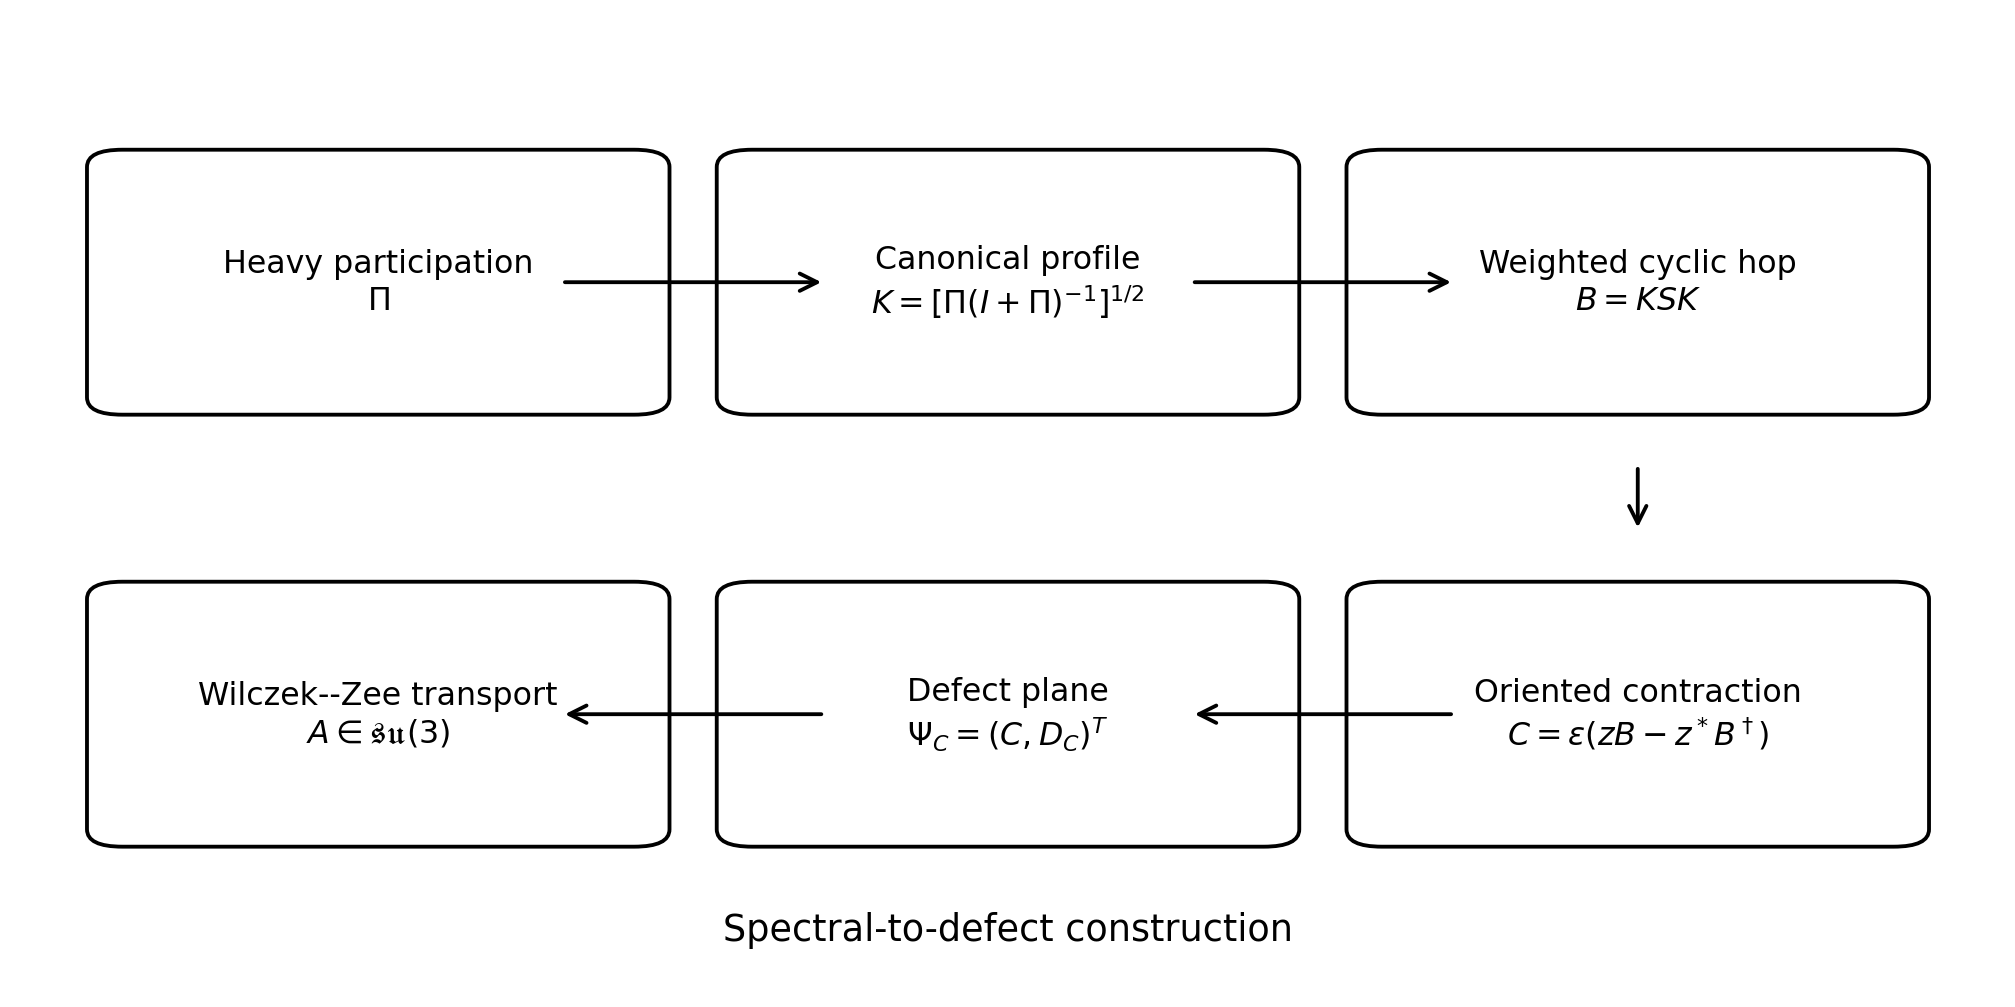
\includegraphics[width=0.98\linewidth]{figures/fig1_pipeline.png}
\caption{The spectral-to-defect chain studied in this paper. The new claim concerns the specific bridge between the standard ingredients, not the individual existence of unitary dilation or Wilczek--Zee holonomy.}
\label{fig:pipeline}
\end{figure}

Our main exact results are: (i) the compressed weighted hop is a strict contraction; (ii) its generic one-step unitary completion is minimally $3+3$; (iii) the anti-Hermitian defect family has an exactly traceless canonical connection; (iv) the isotropic limit is exactly flat; and (v) a rational finite-jet certificate proves generic full $\mathfrak{su}(3)$ holonomy on an open dense set. The unresolved physical problem is not algebraic capacity but path selection: full $SU(3)$ holonomy can generate too many matrices unless the microscopic theory selects a unique transport contour.

\section{Heavy participation and canonical normalization}
Let a three-dimensional light-family sector couple to a gapped heavy sector. Denote by $T$ the heavy-participation amplitude after eliminating the heavy variables at a fixed energy scale and define the positive light-space metric
\begin{equation}
\Pi = TT^\dagger\ge 0.
\end{equation}
The light norm is corrected to $G=I+\Pi$. Canonical normalization gives
\begin{equation}
T_c=(I+\Pi)^{-1/2}T.
\end{equation}
Hence
\begin{equation}
T_cT_c^\dagger=\Pi(I+\Pi)^{-1}.
\end{equation}
We define the positive contraction
\begin{equation}
K=\big[\Pi(I+\Pi)^{-1}\big]^{1/2}.
\label{eq:K}
\end{equation}
If $\pi_i$ is an eigenvalue of $\Pi$, then
\begin{equation}
k_i=\sqrt{\frac{\pi_i}{1+\pi_i}},\qquad 0\le k_i<1
\end{equation}
for every finite $\pi_i$.

A polar decomposition of the normalized participation map reads $T_c=KU_T$. The operator $K$ contains participation strengths, whereas $U_T$ contains a relative heavy-family frame. The construction below is predictive only if the microscopic theory fixes $U_T$, makes it pure convention, or otherwise prevents it from becoming an independent flavor compass.

\section{Compression of a cyclic heavy hop}
Assume a unitary cyclic structural operator $S_H$ acting on a participating heavy triplet. The light compression of one heavy excursion containing this hop is
\begin{equation}
B=T_cS_HT_c^\dagger=K(U_TS_HU_T^\dagger)K.
\end{equation}
In a structurally locked basis, write $S_{\mathrm{eff}}=S$ with $S^3=I$ and choose
\begin{equation}
S=\begin{pmatrix}0&1&0\\0&0&1\\1&0&0\end{pmatrix},\qquad K=\mathrm{diag}(k_1,k_2,k_3).
\end{equation}
Then
\begin{equation}
B=KSK=\begin{pmatrix}0&a&0\\0&0&b\\c&0&0\end{pmatrix},
\quad a=k_1k_2,\quad b=k_2k_3,\quad c=k_3k_1.
\label{eq:B}
\end{equation}
The weighting has a direct participation interpretation: every directed edge pays one participation factor at departure and one at arrival (Fig.~\ref{fig:cycle}).

\begin{figure}[H]
\centering
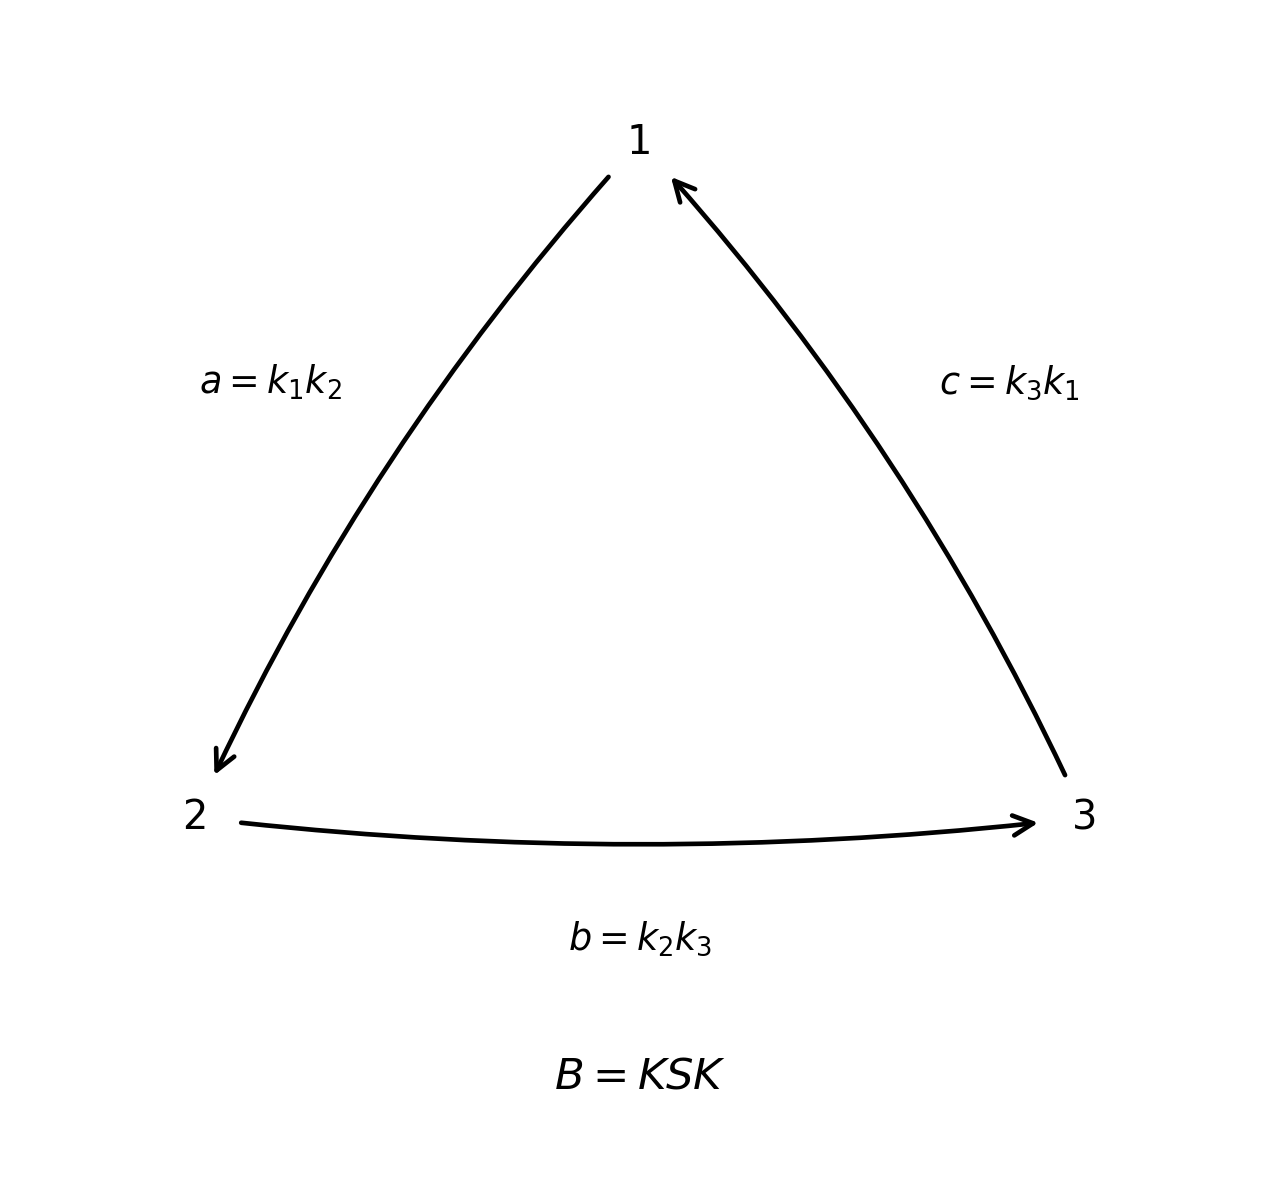
\includegraphics[width=0.53\linewidth]{figures/fig2_cycle.png}
\caption{Weighted cyclic compression $B=KSK$. Spectral anisotropy enters through the three edge products $a,b,c$.}
\label{fig:cycle}
\end{figure}

Direct multiplication yields
\begin{align}
BB^\dagger&=\mathrm{diag}(a^2,b^2,c^2),\\
B^\dagger B&=\mathrm{diag}(c^2,a^2,b^2),\\
[B,B^\dagger]&=\mathrm{diag}(a^2-c^2,b^2-a^2,c^2-b^2).
\label{eq:comm}
\end{align}
For positive weights, $B$ is normal if and only if $a=b=c$. Since $\|S\|=1$ and $\|K\|<1$, $B$ is generically a strict contraction,
\begin{equation}
\|B\|\le \|K\|^2<1.
\end{equation}
Thus $KSK$ is not itself an $SU(3)$ family link. It is a compressed hop whose missing norm must be stored in a complementary sector.

\section{Minimal one-step unitary completion}
Suppose a unitary operator on $\mathbb{C}^3\oplus\mathbb{C}^m$ contains $B$ in its visible block,
\begin{equation}
U=\begin{pmatrix}B&A\\C&D\end{pmatrix}.
\end{equation}
Column unitarity requires
\begin{equation}
C^\dagger C=I-B^\dagger B.
\end{equation}
Therefore
\begin{equation}
m\ge \mathrm{rank}(I-B^\dagger B).
\end{equation}
For a generic strict weighted cycle the right-hand side equals three. Hence three complementary dimensions are necessary. They are sufficient via the Julia operator
\begin{equation}
J_B=\begin{pmatrix}B&D_{B^\dagger}\\D_B&-B^\dagger\end{pmatrix},
\end{equation}
where
\begin{equation}
D_B=(I-B^\dagger B)^{1/2},\qquad D_{B^\dagger}=(I-BB^\dagger)^{1/2}.
\end{equation}
This is a standard one-step unitary completion \cite{SzNagy2010,JulaModern2021}, but in the present construction it has a specific consequence:
\begin{equation}
\boxed{\text{a generic weighted three-family contraction requires a minimal }3+3\text{ one-step completion}.}
\end{equation}
This statement does not imply six fundamental internal dimensions and should not be confused with a power dilation reproducing $B^n$ for every $n$.

The first three columns of $J_B$ define the orthonormal frame
\begin{equation}
\Psi_B=\begin{pmatrix}B\\D_B\end{pmatrix},\qquad \Psi_B^\dagger\Psi_B=I.
\end{equation}
Thus $B$ canonically determines a plane $W_B\in \mathrm{Gr}(3,6)$.

\section{Why the one-way contraction is not enough}
The canonical connection of the $B$-plane is
\begin{equation}
A_B=\Psi_B^\dagger d\Psi_B=B^\dagger dB+D_BdD_B.
\end{equation}
Taking the trace and differentiating $D_B^2=I-B^\dagger B$ gives the exact identity
\begin{equation}
\mathrm{Tr}\,A_B=\frac12\mathrm{Tr}(B^\dagger dB-dB^\dagger B).
\label{eq:traceB}
\end{equation}
The determinant-line curvature is
\begin{equation}
\mathrm{Tr}\,F_B=\mathrm{Tr}(dB^\dagger\wedge dB).
\end{equation}
Hence ambient unitarity does not automatically reduce the selected three-plane from $U(3)$ to $SU(3)$. A determinant-one family connection requires additional structure.

\section{Anti-Hermitian defect construction}
The physically oriented combination of a hop and its reverse is naturally anti-Hermitian. Let
\begin{equation}
C(z)=\epsilon\left(zB-z^*B^\dagger\right),\qquad C^\dagger=-C,
\label{eq:C}
\end{equation}
where $\epsilon$ is real and the domain is restricted so that $\|C\|<1$. Define
\begin{equation}
D_C=(I-C^\dagger C)^{1/2}=(I+C^2)^{1/2},
\end{equation}
and the rank-three frame
\begin{equation}
\Psi_C=\begin{pmatrix}C\\D_C\end{pmatrix}.
\end{equation}
Figure~\ref{fig:defect} summarizes the $3+3$ embedding.

\begin{figure}[H]
\centering
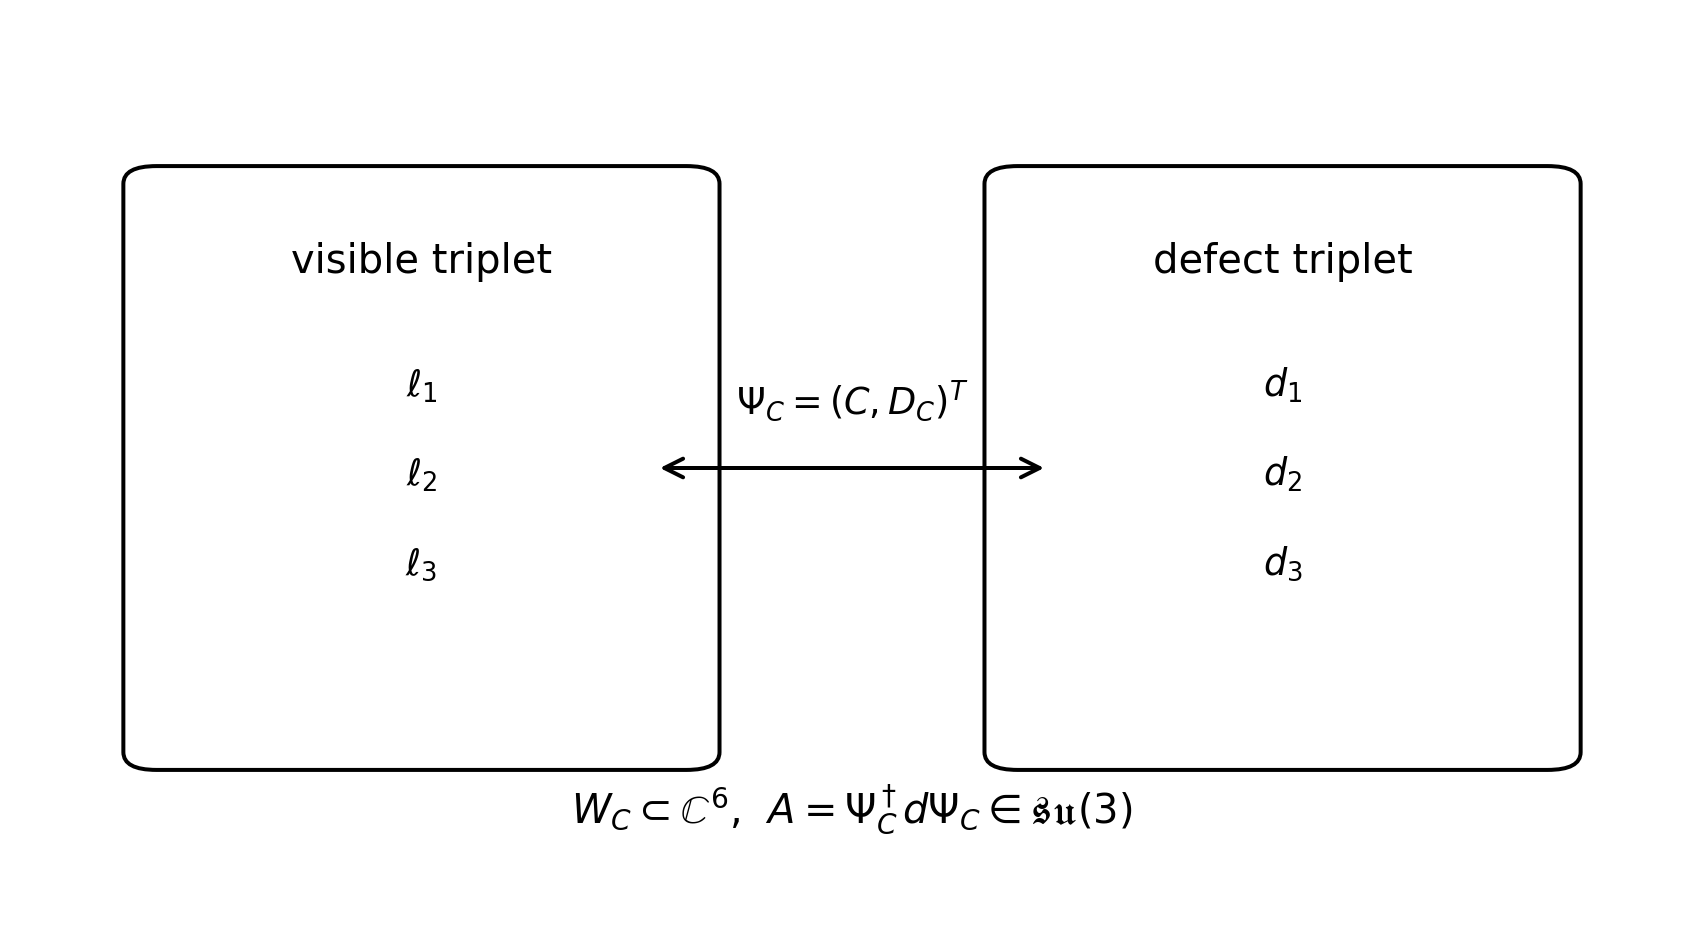
\includegraphics[width=0.70\linewidth]{figures/fig3_defect.png}
\caption{The anti-Hermitian contraction defines a rank-three plane in $\mathbb{C}^6$. The canonical connection of this special family is exactly traceless.}
\label{fig:defect}
\end{figure}

\begin{theorem}[Exact volume lock]
For every smooth family of strict anti-Hermitian contractions $C$, the canonical defect-plane connection
\begin{equation}
A=\Psi_C^\dagger d\Psi_C
\end{equation}
is exactly $\mathfrak{su}(3)$-valued.
\end{theorem}

\begin{proof}
Because $C^\dagger=-C$,
\begin{equation}
A=-CdC+D_CdD_C.
\end{equation}
Differentiating $D_C^2=I+C^2$ gives
\begin{equation}
D_CdD_C+dD_CD_C=CdC+dCC.
\end{equation}
Rearranging,
\begin{equation}
A=\frac12\left([dC,C]+[D_C,dD_C]\right).
\label{eq:Acomm}
\end{equation}
Both terms are commutators, so $\mathrm{Tr}\,A=0$. Anti-Hermiticity follows from $\Psi_C^\dagger\Psi_C=I$. Hence $A\in\mathfrak{su}(3)$.
\end{proof}

This is the central determinant-lock result. No $U(1)$ part is subtracted by hand. If the global transition functions are determinant-one, every corresponding parallel transporter lies in $SU(3)$.

\section{Curvature and spectral anisotropy}
At the symmetric point $z=0$ one has $C=0$, $D_C=I$, and $A=0$. The curvature reduces to
\begin{equation}
F(0)=dC^\dagger\wedge dC=\epsilon^2[B,B^\dagger]dz\wedge dz^*,
\label{eq:F0}
\end{equation}
up to the orientation convention of the complex parameter plane. By Eq.~\eqref{eq:comm}, the same participation anisotropy that makes $B$ non-normal becomes the leading curvature direction.

The isotropic limit is stronger than merely having zero leading curvature.

\begin{theorem}[Isotropic triviality]
If $a=b=c$, the entire anti-Hermitian defect connection vanishes identically.
\end{theorem}

\begin{proof}
For $a=b=c$, $B$ and $B^\dagger$ commute. Every $C(z)$ lies in the same commuting algebra, so $[dC,C]=0$. Since $D_C$ is a function of $C$, $[D_C,dD_C]=0$. Equation~\eqref{eq:Acomm} therefore gives $A=0$.
\end{proof}

Thus heavy spectral isotropy is an exact no-holonomy point of the construction.

\section{Generic full $\mathfrak{su}(3)$ holonomy}
Exact trace locking only shows $\mathrm{Hol}(A)\subseteq SU(3)$. To determine whether the connection is generically confined to a proper subgroup, write $z=x+iy$ and
\begin{equation}
C=xP+yQ,
\qquad P=\epsilon(B-B^\dagger),\qquad Q=i\epsilon(B+B^\dagger).
\end{equation}
The connection is odd and the curvature is even under $(x,y)\mapsto(-x,-y)$, so
\begin{equation}
F_{xy}=F_0+x^2F_{20}+xyF_{11}+y^2F_{02}+O(r^4).
\end{equation}
The leading term is Cartan-valued,
\begin{equation}
F_0=2i\epsilon^2\,\mathrm{diag}(c^2-a^2,a^2-b^2,b^2-c^2).
\end{equation}
At second order the off-diagonal root sectors appear with characteristic coefficients
\begin{equation}
bc(c^2-b^2),\qquad ab(b^2-a^2),\qquad ac(a^2-c^2).
\end{equation}
Hence a complete anisotropic cycle activates all three root pairs. Commutators with $F_0$ separate the roots, while root-root commutators regenerate the two Cartan directions.

The following exact certificate converts this observation into a generic result.

\begin{theorem}[Generic full holonomy algebra]
For the weighted cyclic anti-Hermitian defect family, the curvature-jet Lie algebra is $\mathfrak{su}(3)$ on a nonempty open dense subset of the admissible weight space.
\end{theorem}

\begin{proof}[Proof sketch]
Choose the admissible rational profile $K=\mathrm{diag}(1/2,1/3,1/4)$, so $(a,b,c)=(1/6,1/12,1/8)$. In the real basis
\[
\{H_1,H_2,X_{12},Y_{12},X_{13},Y_{13},X_{23},Y_{23}\}
\]
of $\mathfrak{su}(3)$, take the eight Lie generators
\[
F_0,\ F_{20},\ F_{11},\ F_{02},\ [F_0,F_{20}],\ [F_0,F_{11}],\ [F_{20},F_{11}],\ [F_{20},F_{02}].
\]
After independent nonzero rational rescalings of the columns, their coordinate matrix is
\[
M=\begin{pmatrix}
7&28&0&28&0&0&693&0\\
-5&-80&0&-80&0&0&180&0\\
0&0&5&0&95&0&0&85\\
0&-15&0&15&0&95&-340&0\\
0&0&16&0&-32&0&0&104\\
0&48&0&-48&0&32&416&0\\
0&0&14&0&-238&0&0&-329\\
0&-42&0&42&0&-238&1316&0
\end{pmatrix}.
\]
Its exact determinant is
\begin{equation}
\det M=2{,}822{,}930{,}611{,}200{,}000\ne0.
\end{equation}
Therefore the generated real Lie algebra has dimension eight and equals $\mathfrak{su}(3)$ at this point. The same determinant before specialization is an algebraic function of $a,b,c$ and is not identically zero. Its nonvanishing set is open and dense in the ordinary topology (and Zariski open in the algebraic parameter space), proving generic rank eight.
\end{proof}

By Ambrose--Singer \cite{AmbroseSinger1953}, the restricted holonomy algebra is therefore generically $\mathfrak{su}(3)$, and the connected restricted holonomy group is $SU(3)$.

\section{Exceptional loci}
The theorem is generic rather than universal. Several exceptional loci are explicit:
\begin{enumerate}[leftmargin=*]
\item $a=b=c$: exact flatness.
\item $abc=0$: the cycle is broken and cannot generate the full root system.
\item pairwise equalities such as $a^2=b^2$: at least one second-jet root coefficient vanishes and the holonomy reduces to a proper subgroup.
\end{enumerate}
Additional algebraic exceptional hypersurfaces may be present in the full discriminant. Their complete symbolic factorization is a natural mathematical follow-up.

\section{Interpretation as family transport}
Suppose two chiral sectors receive open parallel transports $L_u,L_d\in SU(3)$ from the defect connection, and write
\begin{equation}
Y_u=L_uD_u,\qquad Y_d=L_dD_d,
\end{equation}
with $D_u,D_d$ positive diagonal. The relative weak-mixing matrix is
\begin{equation}
V=L_u^\dagger L_d.
\end{equation}
The construction has sufficient kinematic capacity for a generic $SU(3)$ family rotation. However, full holonomy is not a prediction of the CKM matrix: a freely chosen contour can generate too much freedom. A predictive ultraviolet model must derive the physical path or discrete sequence of planes independently of flavor data.

The standard weak-CP invariant is basis-independent and may be expressed through the Jarlskog commutator invariant \cite{Jarlskog1985}. The present construction does not yet predict its observed value.

\section{Determinant lock and strong-CP scope}
Because every open geometric family transporter produced by the exact defect connection has determinant one,
\begin{equation}
\det L_f=1.
\end{equation}
Consequently, left multiplication by the geometric orientation does not itself shift $\arg\det Y_f$ when the reference determinant is real and positive. This is potentially useful in determinant-based weak/strong-CP separation mechanisms reminiscent of the structural logic of Nelson--Barr models \cite{Nelson1984,Barr1984}.

It is crucial not to overstate this point. The physical strong parameter also depends on the ultraviolet QCD theta angle, anomalous chiral transformations, heavy-threshold determinants and possible higher-dimensional CP-odd operators. We therefore use the term \emph{determinant lock}, not \emph{solution of strong CP}.

\section{Relation to prior work and novelty}
Every individual mathematical ingredient used above has precedent. Berry and Wilczek--Zee phases are established \cite{Berry1984,WilczekZee1984}; canonical Grassmann/Stiefel holonomy and the isoholonomic problem are standard \cite{Tanimura2005}; three-dimensional non-Abelian holonomy has been realized experimentally \cite{Neef2023}; unitary completion of contractions is standard operator theory \cite{SzNagy2010,JulaModern2021}; and a geometric interpretation of CKM CP has previously been proposed \cite{Fanchiotti2017}. A recent non-peer-reviewed preprint also reports a rank-three eigenbundle whose curvature closes to $\mathfrak{su}(3)$ in a very different deterministic lattice substrate \cite{Molzberger2026}.

Accordingly, we do not claim novelty for ``$SU(3)$ holonomy'' in isolation. The candidate novelty is the specific spectral-to-defect bridge
\begin{equation}
\Pi\longrightarrow K\longrightarrow KSK\longrightarrow C(z)\longrightarrow \Psi_C\longrightarrow A\in\mathfrak{su}(3),
\end{equation}
and the causal relation between spectral anisotropy, non-normality, curvature and generic full holonomy.

To our knowledge, the complete chain has not previously been developed as a mechanism for family transport. This is a literature-based statement, not a formal proof of priority, and should be updated before submission.

\begin{table}[H]
\centering
\small
\caption{Novelty boundary.}
\begin{tabular}{p{0.34\linewidth}p{0.25\linewidth}p{0.31\linewidth}}
\toprule
Component & Prior status & Status here\\
\midrule
Julia/defect completion of a contraction & Established & Structural input\\
Stiefel connection $A=V^\dagger dV$ & Established & Structural input\\
Non-Abelian rank-three holonomy & Established & Not claimed in isolation\\
$\Pi\to K\to KSK$ participation chain & No close precedent identified & Candidate novelty\\
Anti-Hermitian defect family with exact trace lock in this chain & No close precedent identified & Central exact construction\\
Anisotropy-driven transition from flatness to generic full $\mathfrak{su}(3)$ & No close precedent identified in this form & Central generic result\\
CKM prediction & Not achieved & Open\\
Full strong-CP solution & Not achieved & Open\\
\bottomrule
\end{tabular}
\end{table}

\section{Falsifiability and open problems}
The mechanism can fail in sharply separable ways:
\begin{enumerate}[leftmargin=*]
\item \textbf{Spectral origin:} $K$ must be derived from a heavy spectrum rather than inferred from CKM.
\item \textbf{Structural origin:} the cyclic operator $S$ must be fixed by microscopic relational structure.
\item \textbf{Frame closure:} the polar unitary $U_T$ must not be an independent family compass.
\item \textbf{Physical base:} the parameter $z$ must be identified with an actual configuration-space or discrete relational variable without introducing uncontrolled local fluctuation spurions.
\item \textbf{Path selection:} the physical contour must be derived; full holonomy capacity is not flavor predictivity.
\item \textbf{Observer quotient:} additional Wilson-loop matrices must not survive as independent low-energy flavor observers.
\item \textbf{Strong-CP completion:} determinant locking must survive anomalies, thresholds and higher-dimensional operators.
\end{enumerate}
These conditions define a research program rather than a completed ultraviolet theory.

\section{Discussion}
The construction reveals a compact causal chain. A positive heavy participation metric becomes a bounded profile $K$ after canonical normalization. A fixed cyclic hop becomes non-normal when sandwiched between unequal participation amplitudes. That non-normality reappears as leading curvature of a defect-plane connection. The anti-Hermitian orientation simultaneously removes the determinant-line $U(1)$ without subtracting it by hand. Higher curvature jets then recover the off-diagonal root directions needed for generic full $SU(3)$ holonomy.

The same anisotropy therefore has two roles: it determines the edge hierarchy and breaks the geometric symmetry sufficiently to produce non-Abelian holonomy. The isotropic limit provides a particularly sharp negative test: the connection is not merely smaller but exactly trivial.

The minimal $3+3$ embedding should be interpreted carefully. It is a theorem about one-step conservative completion of a full-defect rank-three contraction, not a derivation of six spacetime or internal dimensions. Likewise, full $SU(3)$ holonomy is a capacity result, not a prediction of a particular family matrix.

\section{Conclusion}
We have constructed a rank-three defect geometry linking heavy spectral participation to exact determinant-one non-Abelian holonomy. The main results are:
\begin{enumerate}[leftmargin=*]
\item canonical heavy participation defines the positive contraction $K=[\Pi(I+\Pi)^{-1}]^{1/2}$;
\item a fixed cyclic heavy hop compresses to $B=KSK$;
\item generic finite participation makes $B$ a strict non-normal contraction;
\item its one-step unitary completion requires a minimal $3+3$ ambient space;
\item the anti-Hermitian contraction $C=\epsilon(zB-z^*B^\dagger)$ defines a defect plane whose canonical connection is exactly traceless;
\item the leading curvature is $F(0)=\epsilon^2[B,B^\dagger]dz\wedge dz^*$;
\item the isotropic cycle is exactly flat;
\item an exact rational finite-jet certificate proves generic full $\mathfrak{su}(3)$ holonomy on an open dense set.
\end{enumerate}
The unresolved bottleneck is physical path selection. A complete family theory must derive the heavy spectrum, the cyclic structural hop and the transport path independently of CKM data, and a complete strong-CP model must additionally control the QCD theta term, anomalies and heavy matching. The present work therefore offers a falsifiable operator-geometric mechanism rather than a completed theory of flavor.

\appendix
\section{Second curvature jet}
For reproducibility, set $\epsilon=1$ in this appendix and write $z=x+iy$. The curvature through second order takes
\begin{equation}
F_{xy}=F_0+x^2F_{20}+xyF_{11}+y^2F_{02}+O(r^4),
\end{equation}
with
\begin{equation}
F_0=2i\,\mathrm{diag}(c^2-a^2,a^2-b^2,b^2-c^2),
\end{equation}
and
\begin{equation}
F_{20}=i\begin{pmatrix}
2b^2(c^2-a^2)&bc(c^2-b^2)&ab(b^2-a^2)\\
bc(c^2-b^2)&2c^2(a^2-b^2)&ac(a^2-c^2)\\
ab(b^2-a^2)&ac(a^2-c^2)&2a^2(b^2-c^2)
\end{pmatrix},
\end{equation}
\begin{equation}
F_{11}=2\begin{pmatrix}
0&bc(c^2-b^2)&ab(a^2-b^2)\\
-bc(c^2-b^2)&0&ac(a^2-c^2)\\
-ab(a^2-b^2)&-ac(a^2-c^2)&0
\end{pmatrix},
\end{equation}
\begin{equation}
F_{02}=i\begin{pmatrix}
2b^2(c^2-a^2)&-bc(c^2-b^2)&-ab(b^2-a^2)\\
-bc(c^2-b^2)&2c^2(a^2-b^2)&-ac(a^2-c^2)\\
-ab(b^2-a^2)&-ac(a^2-c^2)&2a^2(b^2-c^2)
\end{pmatrix}.
\end{equation}
The expressions follow by expanding $D_C=(I+C^2)^{1/2}=I+\tfrac12C^2-\tfrac18C^4+\cdots$, inserting into Eq.~\eqref{eq:Acomm}, and retaining the terms required for curvature through order $r^2$.

\section{Exact rank-eight certificate}
At $K=\mathrm{diag}(1/2,1/3,1/4)$, define the $\mathfrak{su}(3)$ basis
\begin{align}
H_1&=i\,\mathrm{diag}(1,-1,0),& H_2&=i\,\mathrm{diag}(0,1,-1),\\
X_{ij}&=E_{ij}-E_{ji},&Y_{ij}&=i(E_{ij}+E_{ji}).
\end{align}
Using the ordered basis $(H_1,H_2,X_{12},Y_{12},X_{13},Y_{13},X_{23},Y_{23})$, the independently rescaled columns of the eight generators used in the proof give the integer matrix printed in the main theorem. Its determinant was verified exactly with integer arithmetic. This certificate is sufficient to establish that the generic rank determinant is not the zero polynomial.

\section{Reproducibility pseudocode}
A symbolic implementation requires only matrix arithmetic:
\begin{enumerate}[leftmargin=*]
\item construct symbolic $B(a,b,c)$;
\item set $P=B-B^\dagger$, $Q=i(B+B^\dagger)$ and $C=xP+yQ$;
\item expand $D=(I+C^2)^{1/2}$ to fourth order in $C$;
\item compute $A=\tfrac12([dC,C]+[D,dD])$;
\item compute $F=dA+A\wedge A$ and extract $F_0,F_{20},F_{11},F_{02}$;
\item specialize to $(a,b,c)=(1/6,1/12,1/8)$;
\item form the eight Lie words listed in the theorem;
\item express them in the real $\mathfrak{su}(3)$ basis and evaluate the determinant exactly.
\end{enumerate}
The accompanying source bundle includes a short symbolic verification script implementing this calculation.

\section{Claim hierarchy}
For clarity, the manuscript separates three levels of statement.

\paragraph{Exact within the model.} Equations \eqref{eq:K}--\eqref{eq:F0}, minimal one-step $3+3$ completion, exact trace lock, isotropic triviality, and the rational rank-eight certificate.

\paragraph{Generic theorem.} Full $\mathfrak{su}(3)$ curvature-jet closure on an open dense subset of weight space.

\paragraph{Open physical interpretation.} Derivation of the Standard Model flavor paths, numerical CKM prediction, the origin of three families and a complete ultraviolet strong-CP solution.

\begin{thebibliography}{99}
\bibitem{Berry1984} M. V. Berry, ``Quantal phase factors accompanying adiabatic changes,'' \emph{Proc. R. Soc. Lond. A} \textbf{392}, 45--57 (1984), doi:10.1098/rspa.1984.0023.
\bibitem{WilczekZee1984} F. Wilczek and A. Zee, ``Appearance of Gauge Structure in Simple Dynamical Systems,'' \emph{Phys. Rev. Lett.} \textbf{52}, 2111--2114 (1984), doi:10.1103/PhysRevLett.52.2111.
\bibitem{AmbroseSinger1953} W. Ambrose and I. M. Singer, ``A Theorem on Holonomy,'' \emph{Trans. Amer. Math. Soc.} \textbf{75}, 428--443 (1953).
\bibitem{Tanimura2005} S. Tanimura, M. Nakahara, and D. Hayashi, ``Exact solutions of the isoholonomic problem and the optimal control problem in holonomic quantum computation,'' \emph{J. Math. Phys.} \textbf{46}, 022101 (2005), doi:10.1063/1.1835545.
\bibitem{Neef2023} V. Neef \emph{et al.}, ``Three-dimensional non-Abelian quantum holonomy,'' \emph{Nature Phys.} \textbf{19}, 30--34 (2023), doi:10.1038/s41567-022-01807-5.
\bibitem{Jarlskog1985} C. Jarlskog, ``Commutator of the Quark Mass Matrices in the Standard Electroweak Model and a Measure of Maximal CP Nonconservation,'' \emph{Phys. Rev. Lett.} \textbf{55}, 1039--1042 (1985), doi:10.1103/PhysRevLett.55.1039.
\bibitem{Nelson1984} A. E. Nelson, ``Naturally weak CP violation,'' \emph{Phys. Lett. B} \textbf{136}, 387--391 (1984), doi:10.1016/0370-2693(84)92025-2.
\bibitem{Barr1984} S. M. Barr, ``Solving the Strong CP Problem without the Peccei-Quinn Symmetry,'' \emph{Phys. Rev. Lett.} \textbf{53}, 329--332 (1984), doi:10.1103/PhysRevLett.53.329.
\bibitem{Fanchiotti2017} H. Fanchiotti, C. A. Garc\'ia Canal, and V. Vento, ``The Geometric Origin of the CP Phase,'' arXiv:1705.08127 [hep-ph] (2017).
\bibitem{Molzberger2026} L. Molzberger, ``Emergent U(1) x SU(3) Gauge Structure and Lorentzian Geometry from a Deterministic Brane-Lattice Substrate,'' Preprints.org (2026), non-peer-reviewed preprint, manuscript 202607.0466.
\bibitem{SzNagy2010} B. Sz.-Nagy, C. Foias, H. Bercovici, and L. Kerchy, \emph{Harmonic Analysis of Operators on Hilbert Space}, Springer (2010).
\bibitem{JulaModern2021} V. Derkach, S. Hassi, and H. de Snoo, ``Generalized Schur--Nevanlinna functions and their realizations,'' \emph{Integral Equations Operator Theory} \textbf{93} (2021), doi:10.1007/s00020-020-02600-w.
\end{thebibliography}
\end{document}
